\documentclass[11pt,a4paper]{article}
\usepackage[utf8]{inputenc}
\usepackage{amsmath,caption,subcaption,graphicx,tikz,floatrow}
\usepackage[hidelinks]{hyperref}
\graphicspath{ {./figures/} }
\usetikzlibrary{automata,arrows,positioning}
\usepackage[margin=2cm]{geometry}
\usepackage{xcolor}
\usepackage[style=apa,
			sorting=nyt,
			date=year,
			bibencoding=utf8,
			isbn=false,
			eprint=false,
			dashed=false,
			uniquelist=false,
			maxbibnames=10,
			minbibnames=1,
			maxcitenames=2,
			uniquename=init,
			giveninits=true,
			useprefix=false,
			minsortnames=1,
			maxsortnames=2]{biblatex}
\renewcommand{\cite}{\parencite}
\captionsetup{labelformat=simple}
\DeclareCaptionSubType[Alph]{figure}
\bibliography{References}
% \newcommand{\Kishore}[1]{{\color{red}[[\textbf{Kishore: }#1]]}}

\title{XCR Draft}
\author{CSB}
\date{January 2023}

\begin{document}

\maketitle

\section{Results}

Having one inactivated X chromosome is a natural state of the cells. Coupled with the fact that X chromosome inactivation is random, these observations indicate an antagonistic relationship between the two X chromosomes \cite{XCI-TS}. However, the observations during iPSC induction contradict such a relationship, owing to the similar activation levels of both the X chromosomes. Therefore, we decided to understand this relationship further using the dynamic X:A data for the chromosomes during partial and complete reactivation of the X-chromosome. We hence generated a mathematical model where each X chromosome is considered as a single entity and asked what nature of interactions between the two chromosomes best explain the observed dynamics in the X:A ratio during partial activation as well as iPSC induction. Without loss of generality, we use the X:A ratio as the level of that particular chromosome.

First, we verified the fits using antagonistic/inhibitory cross-regulation between the two chromosomes. We obtained poor fits (\autoref{IINN}), suggestive of the fact that the model must be modified. We then added activatory self-regulations for each chromosome. The fits obtained by the addition of self-activations are much better than those without self-activations (\autoref{IIAA}). Similarly, the fits obtained by the addition of self-inhibition are also satisfactory (\autoref{IIII-full}). This indicates that some form of self-regulation is necessary to explain the observed dynamics.

% The rationale being that the upregulated X does not lose its upregulation until a threshold activation level of the XCI reached which can be explained by the upregulated chromosome having a self-activation property which serves to contest the inhibition from the inactivation chromosome. 
We then consider all combinations of cross-regulatory links (interactions between the chromosomes) and self-regulatory links (interactions within a chromosome, for example, the expression of some genes on the chromosome enhancing the expression of other genes on the same chromosome via epigenetic modifications) (\autoref{topo}). We generated heatmaps with a color scheme such that the red color indicates a higher $R^2$, indicative of a good fit.

We first tested the self-regulatory connections while the cross-regulatory connections were kept fixed as inhibitory. For the full reactivation case (\autoref{rsq-self-full}), we observe that the connection to $X_a$ being inhibitory gives a good fit regardless of the connection to $X_i$. The case where both are self-activatory also performs well. However, for the case of partial reactivation, where the reactivation follows similar dynamics as iPSC induction but stops mid-way (\autoref{rsq-self-part}, \autoref{IIII-part}), most of these fail, and only the case where both are self-inhibitory performs the best.

Then we tested the cross-regulatory connections while fixing the self-regulatory connection as inhibitory. Here, we observe that the case that best fits the full reactivation case (\autoref{rsq-cross-i-full}) is when both the cross-connections are inhibitory. Whereas, for the partial reactivation case (\autoref{rsq-cross-i-part}), the incoming connection to  $X_a$ being inhibitory gives a better fit, while the connection to $X_i$ being activatory performs slightly better.

Similarly, we also tested the cross-regulatory connections while fixing the self-regulatory connection to be activatory. We find that the incoming connection to $X_i$ does not matter as much for the full reactivation case (\autoref{rsq-cross-a-full}). However, the incoming connection to $X_a$ being inhibitory gives a better fit. Similarly, the incoming connection to $X_a$ being inhibitory for the partial reactivation case (\autoref{rsq-cross-a-part}) gives a better fit, whereas the incoming connection to $X_i$ does not matter as much.

% Although we have cases where certain combinations of regulatory connections fit best, the double cross inhibitory and double self-inhibitory perform reasonably well and consistently across cases, leading us to consider it be the likely interactions (\autoref{IIII-full}, ). 

Our results indicate that the self-inhibition with cross-inhibitory regulation explains the reactivation dynamics consistently well for both partial and full reactivation. Despite the ability of our phenomenological model to explain the observed experimental data, it falls short of revealing the specific mechanisms mediating such interactions among the chromosomes. One possibility is that the cross-inhibition identified above corresponds to competition between the two chromosomes for specific resources and/or interactions mediated by regulatory factors that are pertinent during random X-inactivation \cite{XCI}.

To identify the difference between the two cases (full vs. partial reactivation), we quantified the coefficients of each term which can act as a proxy for the strength of connections (\autoref{IIII-parm}). The cross-inhibition on $X_i$ given by $a_1$ is higher in the case of partial reactivation, whereas the cross-inhibition on $X_a$ given by $a_2$ is lower in the case of partial reactivation. The self-inhibition on $X_a$ given by $b_2$ is higher in the case of partial reactivation, whereas the self-inhibition on $X_i$ is negligible in both cases. This sensitivity analysis indicated the relative role of different interactions in mediating partial versus full reactivation dynamics.

Our model so far has been fit to the mean X:A values at the population level. However, we observe a heterogeneity in the population in the experimental data, i.e., at any time point, there is a fraction of the population that is $X_a, X_i$ and the rest is $X_a, X_r$. Furthermore, this fraction keeps changing over time. We hypothesized that the heterogeneity can be explained by the presence of noise in the system. To test this hypothesis, we added a noise term to our equations and solved them with the parameter set we obtained from our fits. We see here that the addition of noise leads to a fraction of cells reactivating faster than the others in the system, evident by the bimodality (\autoref{IIII-noise}). Hence, our model can also explain the heterogeneity in reactivation in addition to the mean behavior of the population. 

\section{Methods}

\subsection*{Mathematical model describing the population level dynamics of X reactivation}
We have considered the two X-chromosomes as interacting entities, and they are modeled as differential equations given by:
\begin{equation}
    \frac{dX_i}{dt} = \underbrace{a_1\ f(K_1,X_a,n)}_\text{cross} + \underbrace{b_1\ f(K_3,X_i,n)}_\text{self} - \underbrace{c_1 X_i}_\text{decay} 
    \label{Xi-eq}
\end{equation}
\begin{equation}
    \frac{dX_a}{dt} = \underbrace{a_2\ f(K_2,X_i,n)}_\text{cross} + \underbrace{b_2\ f(K_4,X_a,n)}_\text{self} - \underbrace{c_2 X_a}_\text{decay} 
    \label{Xa-eq}
\end{equation}
Where, 
\begin{equation}
    f(K,X,n) = 
    \begin{cases} 
        \frac{{X}^n}{{K}^n+{X}^n} & \text{if activatory}\\
        \frac{{K}^n}{{K}^n+{X}^n} & \text{if inhibitory}\\
        0 & \text{if neutral}
    \end{cases}
\end{equation}

$X_i$ is the expression level of the inactive X given as X:A ratio, $X_a$ is the expression level of the active X given as X:A ratio, $a_1, a_2, b_1, b_2, c_1$ and $c_2$ are the coefficients for cross-regulatory, self-regulatory and decay terms, respectively, $n$ is the hill coefficient, $K_1,K_2,K_3$ and $K_4$ are the half-saturation constants.

\subsection*{Fitting the model to single cell iPSC induction and partial reactivation data}
For the data for full reactivation, we took the data obtained from X-reactivation in iPSC given in \ref{ipsc-data}. Due to lack of data between day 0 to day 8, the starting point for X-reactivation was considered to be day 7 and with the same level corresponding to day 0 in the iPSC data. The mean value for day wise levels of $X_i$ and $X_a$ were considered. The levels for iPSC cells were considered as the levels from day 13 to day 15. For the data for partial reactivation, we assumed a hypothetical case of iPSC reactivation stalling at day 12. The value at day 12 was extrapolated up to day 15. These values match qualitatively with the partial reactivation state in \ref{xen-data} and have been done due to the lack of temporal data.

These equations are fit to the time course data for full and partial reactivation. This was done by minimizing the sum of square error using the \texttt{differential\_evolution} algorithm of \texttt{scipy}. The initial population of parameters is sampled using Sobol sampling. The differential equations are solved using the explicit Runge-Kutta method of order 5(4) with these parameters. Then, the sum of square errors between the solutions evaluated at the given time points and the actual data is calculated. A new parameter set is generated by adding a weighted difference between two randomly chosen parameter sets to a third parameter set, similar to a mutation. Then, it randomly combines parameters from the old set with this new set, similar to crossover. The sum of square errors with this new set of parameters is also evaluated and compared with those of the old parameters. If the values are lower with the new set, they replace the old set in the next generation of the population. This is repeated multiple times until an optimal solution is found \cite{DEalgo}.

\subsection*{Simulating the model with the addition of noise}
For the model with noise, we added a noise term $\eta(t)$ to \autoref{Xi-eq} and \autoref{Xa-eq} where the values are sampled from a normal distribution with mean 0 and standard deviation 1. These were then solved with the fit parameters using explicit Runge-Kutta method of order 5(4).

\subsection*{Code availability}
The code implementing this is available at \url{https://github.com/Harshavardhan-BV/rev-XCI}.

 \printbibliography

 \newgeometry{top=0cm,bottom=0cm,left=2cm,right=2cm}
 
\setcounter{figure}{6}
\begin{figure}[p]
    \centering
    \begin{subfigure}[c]{0.32\textwidth}
        \phantomcaption
        \label{IINN}
    \end{subfigure}
    \begin{subfigure}[c]{0.32\textwidth}
        \phantomcaption
        \label{IIAA}
    \end{subfigure}
    \begin{subfigure}[c]{0.32\textwidth}
        \phantomcaption
        \label{IIII-full}
    \end{subfigure}
    \begin{subfigure}[c]{0.22\textwidth}
        \centering
        % \begin{tikzpicture}[node distance=2.2cm,on grid]
        %     \node[state] (Xi)  {$X_i$};
        %     \node[state] (Xa) [below of=Xi] {$X_a$};
        %     \path[->, thick,>=latex]
        %         (Xi) edge [out=40,in=140,looseness=5] node {}    (Xi)
        %         edge [out=210,in=-210]  node {}    (Xa)
        %         (Xa) edge [out=-140,in=-40,looseness=5] node {}    (Xa)
        %         edge [out=30,in=-30]  node {}    (Xi);
        %     \path[-||, thick,>=latex]
        %     (Xi) edge [out=60,in=120,looseness=4] node {}    (Xi)
        %         edge [out=230,in=-230]  node {}    (Xa)
        %     (Xa) edge [out=-120,in=-60,looseness=4] node {}    (Xa)
        %         edge [out=50,in=-50]  node {}    (Xi);
        % \end{tikzpicture}
        \phantomcaption
        \label{topo}
    \end{subfigure}
    \begin{subfigure}[c]{0.35\textwidth}
        \phantomcaption
        \label{rsq-self-full}
    \end{subfigure}
    \begin{subfigure}[c]{0.35\textwidth}
        \phantomcaption
        \label{rsq-self-part}
    \end{subfigure}
    \begin{subfigure}[c]{0.32\textwidth}
        \phantomcaption
        \label{IIII-part}
    \end{subfigure}
    \begin{subfigure}[c]{0.28\textwidth}
        \phantomcaption
        \label{rsq-cross-i-full}
    \end{subfigure}
    \begin{subfigure}[c]{0.28\textwidth}
        \phantomcaption
        \label{rsq-cross-i-part}
    \end{subfigure}
    \begin{subfigure}[c]{0.32\textwidth}
        \phantomcaption
        \label{IIII-parm}
    \end{subfigure}
    \begin{subfigure}[c]{0.28\textwidth}
        \phantomcaption
        \label{rsq-cross-a-full}
    \end{subfigure}
    \begin{subfigure}[c]{0.28\textwidth}
        \phantomcaption
        \label{rsq-cross-a-part}
    \end{subfigure}
    \begin{subfigure}[c]{0.28\textwidth}
        \phantomcaption
        \label{IIII-noise}
    \end{subfigure}
    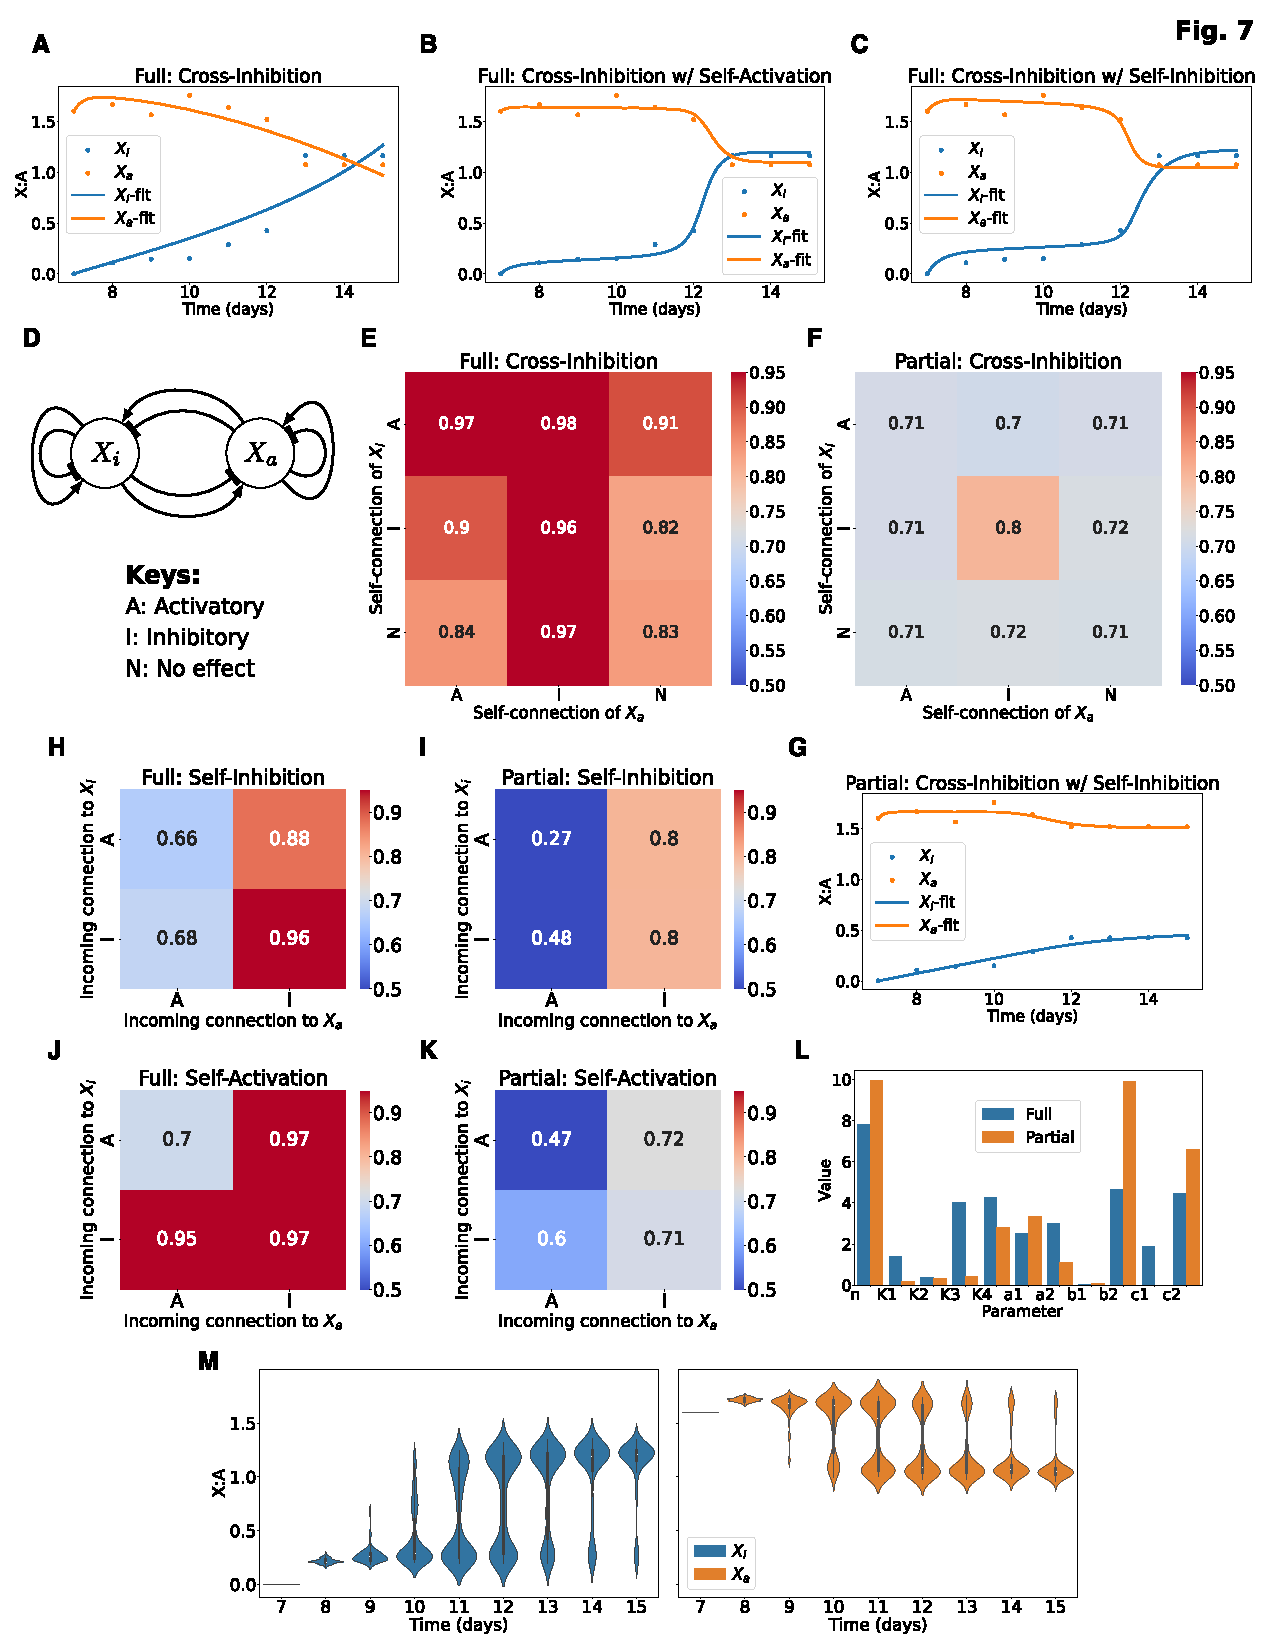
\includegraphics[width=\textwidth]{XCR-model.pdf}
    \caption{\textbf{Phenomenological model to explain partial and full reactivation dynamics}. \subref{IINN}, \subref{IIAA}, \subref{IIII-full}: Fits on full reactivation data with only cross-inhibition, with cross-inhibition and self-activation, and with cross-inhibition and self-inhibition, respectively. \subref{topo}: Schematic of all combinations of regulatory links. \subref{rsq-self-full}, \subref{rsq-self-part}: Heatmaps of $R^2$ for fits testing self-regulatory connections with fixed cross-inhibition on full and partial reactivation data, respectively. \subref{IIII-part}: Fits on partial reactivation data with cross-inhibition and self-inhibition. \subref{rsq-cross-i-full}, \subref{rsq-cross-i-part}: Heatmaps of $R^2$ for fits testing cross-regulatory connections with fixed self-inhibition on full and partial reactivation data, respectively. \subref{rsq-cross-a-full}, \subref{rsq-cross-a-part}: Heatmaps of $R^2$ for fits testing cross-regulatory connections with fixed self-activation on full and partial reactivation data, respectively. \subref{IIII-parm}: Comparison of fit parameters with cross-inhibition and self-inhibition between full and partial reactivation. \subref{IIII-noise}: Time-course distribution of X level on addition of noise to the model.}
\end{figure}
 
\end{document}
